\section{Magnetic Alloy Ringkerne}
Die MA-Ringkerne bestehen aus zwei Teilen. Aus einem inneren Edelstahlring, der als Halterung dient und als nicht magnetisch anzusehen ist, sowie aus einem \"au\ss{}eren Teil, welcher das magnetische Material darstellt. Das magnetische Material ist in diesem Fall Nanoperm~\citep{magnetec2018}. Das Material weist eine sehr hohe Permeabilit\"at in einer Reichweite von 1000 bis 200000 auf. Durch den inneren Ring sind einige Bohrungen durchgef\"uhrt, an denen der Kern innerhalb einer Kavit\"at montiert werden kann.
\begin{figure}[htb]
	\centering
	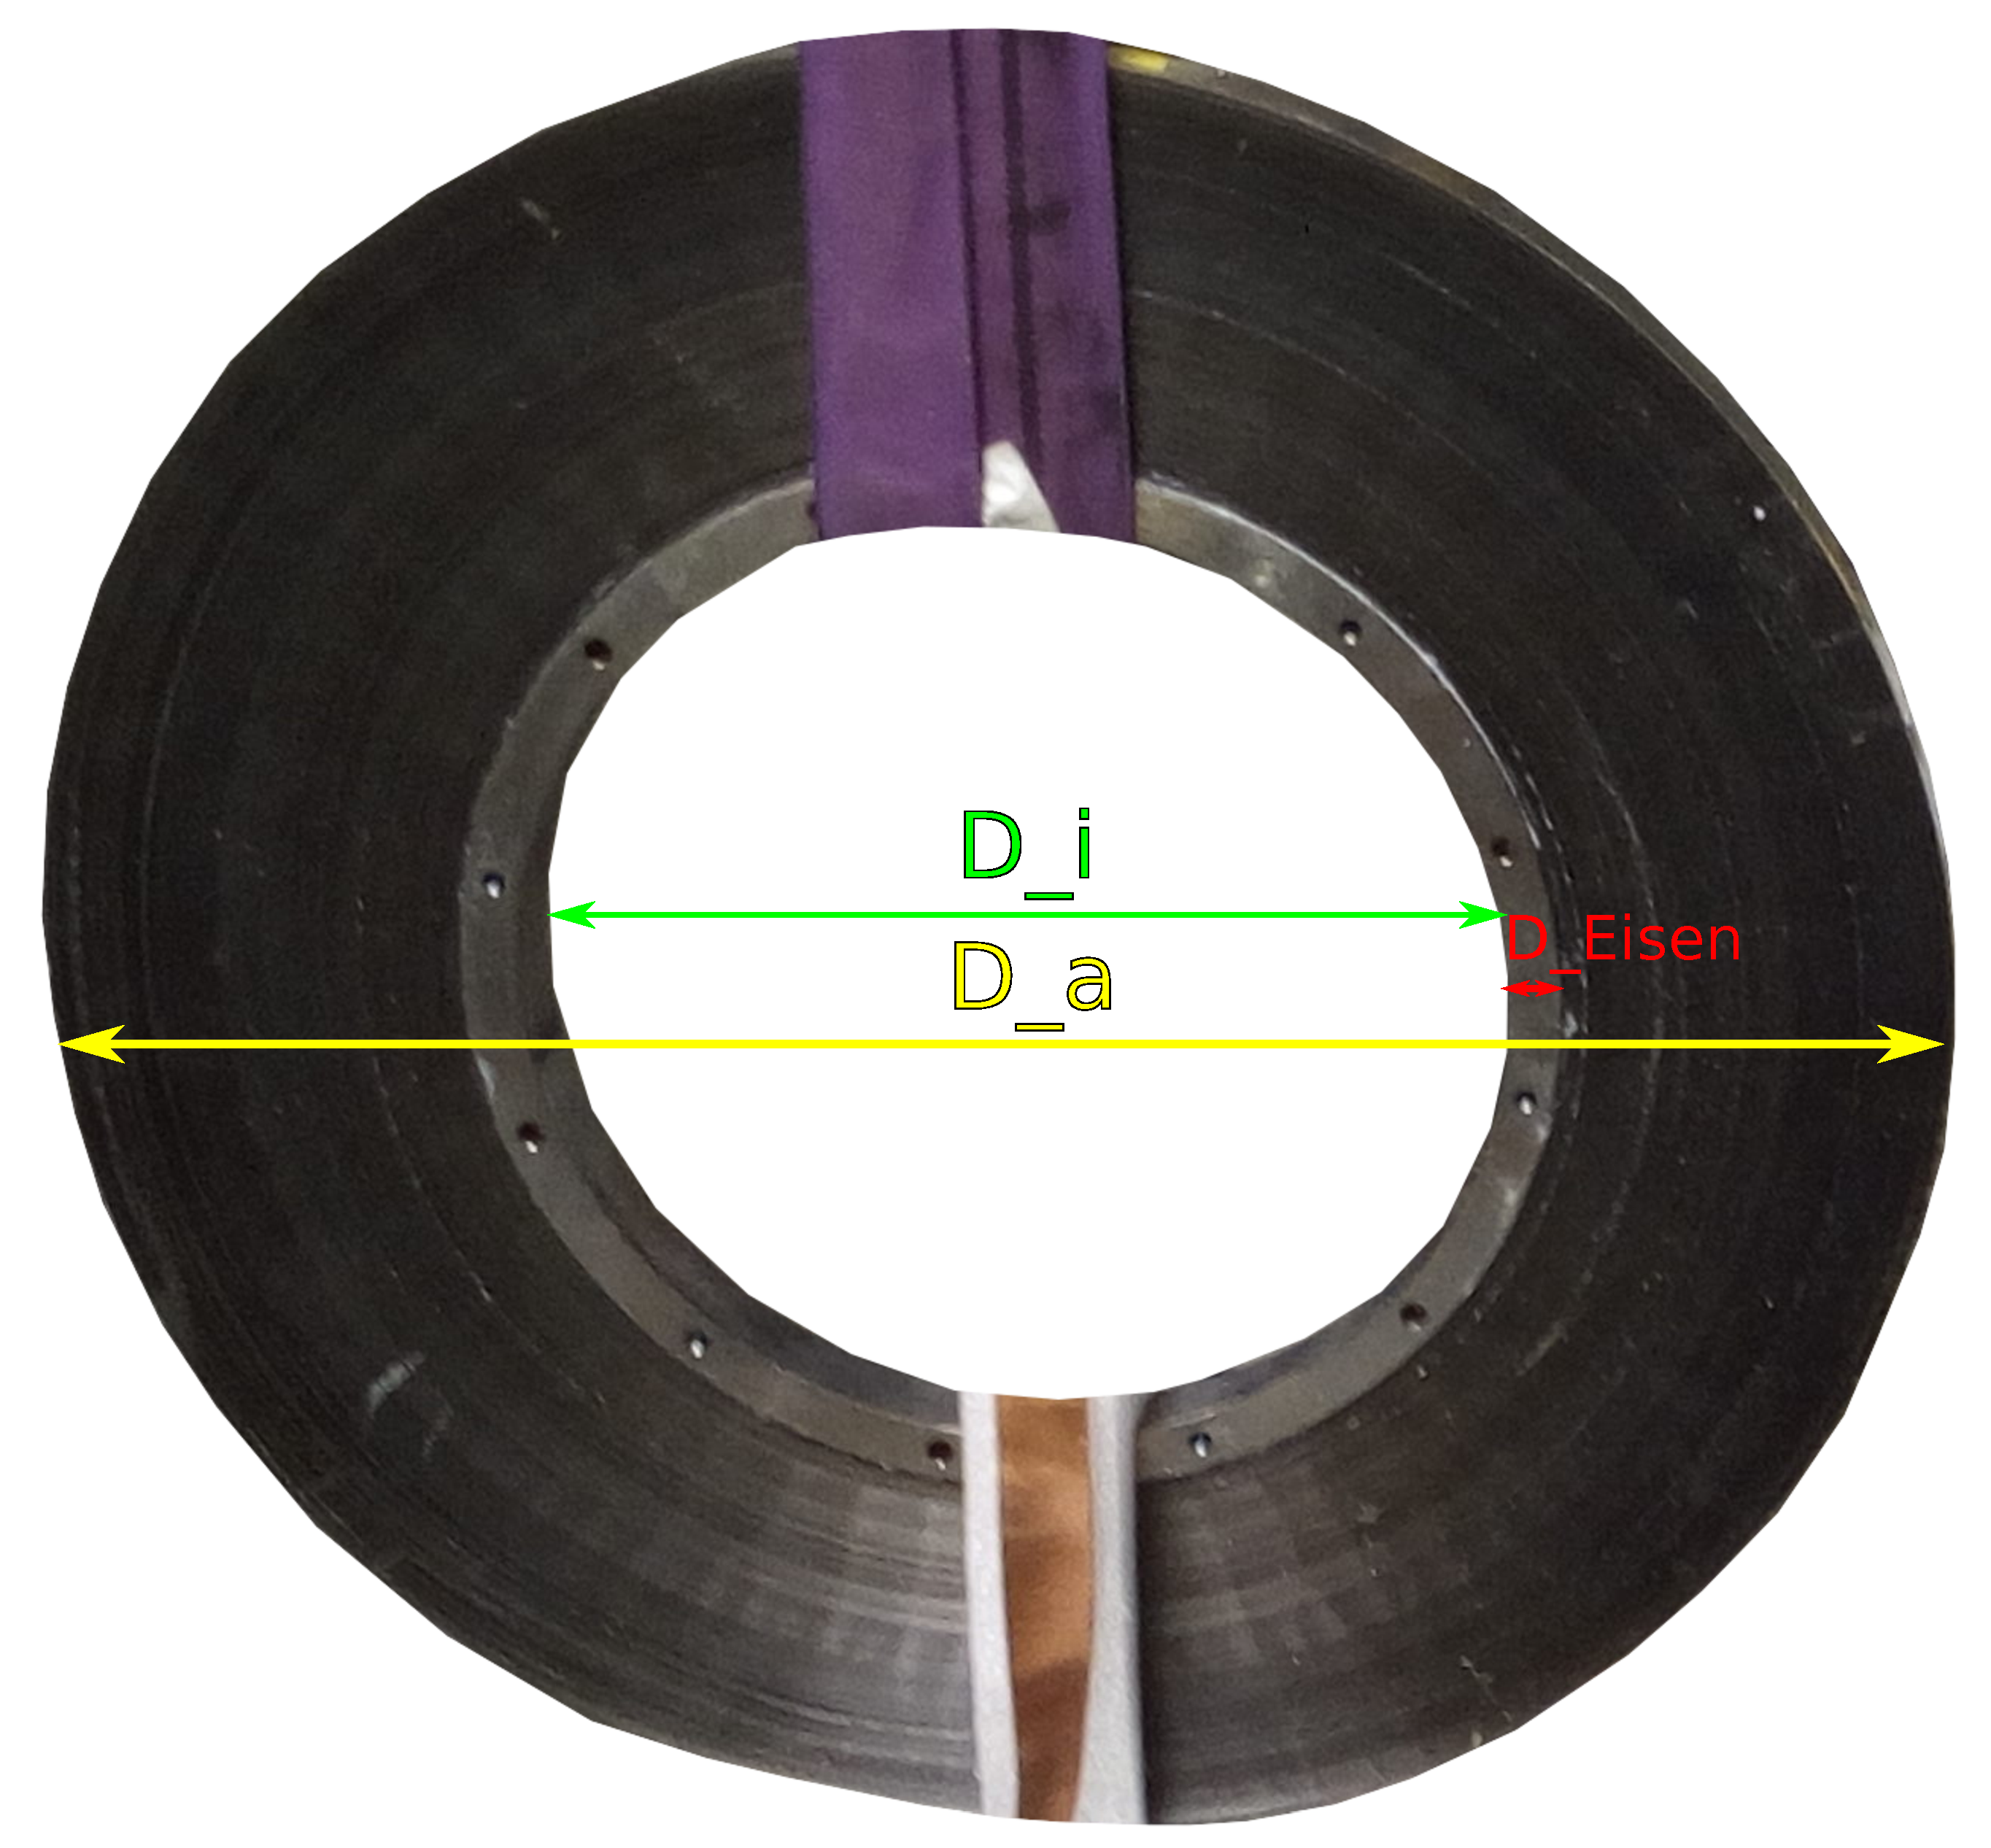
\includegraphics[width=0.6\textwidth]{ringkern.pdf}
	\caption{F\"ur Messungen verwendeter MA-Ringkern mit Abmessungsbezeichnung.}
	\label{fig:ringkern}
\end{figure}
\par
Die genauen Abmessungen des Ringkerns sind in Tabelle~\ref{tab:ringkern} angegeben.
\begin{table}[htb]
	\centering
	\begin{tabular}{| l | l |}
		\hline
		Gr\"o\ss{}e & Wert in Millimeter \\ \hline
		Au\ss{}endurchmesser $D_a$ & 500 \\
		Innendurchmesser $D_i$ & 260 \\
		Breite des Ringkerns & 25 \\
		Breite des Edelstahlrings & 26 \\
		Dicke des Edelstahlrings $D_{Eisen}$ & 15 \\ \hline
	\end{tabular}
	\caption{Abmessungen des verwendeten MA-Ringkerns.}
	\label{tab:ringkern}
\end{table}
